%构思:第一个图切入的时候,说如果不能store的话,那么价格会上下波动。如果可以免费的store,并且是immediately的,那么价格将会成为flat,那么storage将会是没有value的。
%要解释一下为什么production会比较stable,而consumption回很volatile。1.If marginal production costs are increasing with the rate of output 2.there may be adjustment costs, i.e., costs of changing the rate of production. For example, there may be costs of hiring and training new or temporary workers, leasing additional capital, etc.
%heating is the main usage of natural gas。Warm winter and cold winter。
%value strategy is not good. It is kind of fixed.

%Valuation of storage. costs type. continuous time or discrete time. 


%risk-neutral measure. price dynamics.

%moving boundary method. why one dimension is easy.


%%%%%%%%%%%%%%%%%%%%%%%%%%%%%%%%%%%%%%%%%
% Beamer Presentation
% LaTeX Template
% Version 1.0 (10/11/12)
%
% This template has been downloaded from:
% http://www.LaTeXTemplates.com
%
% License:
% CC BY-NC-SA 3.0 (http://creativecommons.org/licenses/by-nc-sa/3.0/)
%
%%%%%%%%%%%%%%%%%%%%%%%%%%%%%%%%%%%%%%%%%

%----------------------------------------------------------------------------------------
%	PACKAGES AND THEMES
%----------------------------------------------------------------------------------------

\documentclass{beamer}

\mode<presentation> {

% The Beamer class comes with a number of default slide themes
% which change the colors and layouts of slides. Below this is a list
% of all the themes, uncomment each in turn to see what they look like.

%\usetheme{default}
%\usetheme{AnnArbor}
%\usetheme{Antibes}
%\usetheme{Bergen}
%\usetheme{Berkeley}
%\usetheme{Berlin}
%\usetheme{Boadilla}
%\usetheme{CambridgeUS}
%\usetheme{Copenhagen}
\usetheme{Darmstadt}
%\usetheme{Dresden}
%\usetheme{Frankfurt}
%\usetheme{Goettingen}
%\usetheme{Hannover}
%\usetheme{Ilmenau}
%\usetheme{JuanLesPins}
%\usetheme{Luebeck}
%\usetheme{Madrid}
%\usetheme{Malmoe}
%\usetheme{Marburg}
%\usetheme{Montpellier}
%\usetheme{PaloAlto}
%\usetheme{Pittsburgh}
%\usetheme{Rochester}
%\usetheme{Singapore}
%\usetheme{Szeged}
%\usetheme{Warsaw}

% As well as themes, the Beamer class has a number of color themes
% for any slide theme. Uncomment each of these in turn to see how it
% changes the colors of your current slide theme.

%\usecolortheme{albatross}
%\usecolortheme{beaver}
%\usecolortheme{beetle}
%\usecolortheme{crane}
%\usecolortheme{dolphin}
%\usecolortheme{dove}
%\usecolortheme{fly}
%\usecolortheme{lily}
%\usecolortheme{orchid}
%\usecolortheme{rose}
%\usecolortheme{seagull}
%\usecolortheme{seahorse}
\usecolortheme{whale}
%\usecolortheme{wolverine}

%\setbeamertemplate{footline} % To remove the footer line in all slides uncomment this line
%\setbeamertemplate{footline}[page number] % To replace the footer line in all slides with a simple slide count uncomment this line

%\setbeamertemplate{navigation symbols}{} % To remove the navigation symbols from the bottom of all slides uncomment this line
}
\usepackage{color}
\usepackage{graphicx} % Allows including images
\usepackage{booktabs} % Allows the use of \toprule, \midrule and \bottomrule in tables
\usepackage{setspace}

\graphicspath{{figures/}}

%----------------------------------------------------------------------------------------
%	TITLE PAGE
%----------------------------------------------------------------------------------------

\title[Short title]{The Valuation of Storage} % The short title appears at the bottom of every slide, the full title is only on the title page

\author{Long Zhao\\ {\footnotesize McCombs School of Business, University of Texas - Austin}} % Your name
\institute[UT Austin] % Your institution as it will appear on the bottom of every slide, may be shorthand to save space
{
 \small{Joint work with Kumar Muthuraman and Stathis Tompaidis}\\ % Your institution for the title page
\medskip
%\textit{longzhao@sutexas.edu} % Your email address
}
\date{\today} % Date, can be changed to a custom date

\begin{document}

\begin{frame}
\titlepage % Print the title page as the first slide
\end{frame}

\section{Motivation}

\begin{frame}
{\bf Examples of Storage}
\begin{itemize}
%  \item Cellphone Battery - Electricity
%  \item Overtime Work - Leisure Time
  \item Silos - Agricultural Commodities
  \item Tanks - Oil
  \item Caverns - Natural Gas 
  \item Lake Reservoirs and Dams - Water $\Rightarrow$ Electricity.          
  \end{itemize}
\end{frame}

\begin{frame}
{\bf Motivation}
\begin{figure}[hbt]
  \includegraphics[width = 8cm]{PriceStorageLevel.pdf}
\end{figure}
\begin{center}
Data comes from U.S. Energy Information Administration.
\end{center}
\end{frame}



\begin{frame}
{\bf Historical Prices}
\begin{figure}[hbt]
  \includegraphics[width = 8cm]{PriceNG.pdf}
\end{figure}
\begin{center}
Data comes from U.S. Energy Information Administration.
\end{center}
\end{frame}

\begin{frame}
{\bf Future Prices}
\only<1>{\begin{figure}[hbt]
  \includegraphics[width = 8cm]{FuturePrices.pdf}
\end{figure}}
\begin{center}
Data comes from U.S. Energy Information Administration.
\end{center}
\end{frame}

\begin{frame}
{\bf Future Prices}
\only<1>{\begin{figure}[hbt]
  \includegraphics[width = 8cm]{FuturePrices14.pdf}
\end{figure}}
\begin{center}
Data comes from U.S. Energy Information Administration.
\end{center}
\end{frame}

\begin{frame}
{\bf Price Dynamics}

      \begin{itemize}
      \item Schwartz (1997) % The first model is a simple one-factor model in which the logarithm of the spot price of the commodity is assumed to follow a mean reverting process.
      % The second model takes into account a second stochastic factor, the convenience yield of the commodity, which is assumed to follow a mean reverting process.
      % The third model also includes stochastic interest rates.
      % For copper data, three models are of the same prediction level. For oil data, 2nd and 3rd are significantly better than the 1st.
      \item Schwartz and Smith (2000)
      %The short-Term/Long term model. Logarithm of the spot price is a mean reverting spot process with a stochastic mean. Logarithm of the spot price is decomposed into two parts short term deviations and equilibrium level. First one is OU process and the second one is a drifted brownian motion. 
      \item Routledge, Seppi and Spatt(2000)
      % Rather than exogenously assuming stochastic processes for spot prices and convenience yields, we derive the spot and forward price processes induced by a mean-reverting immediate use net- demand process and the resulting equilibrium inventory dynamics.
      \item Jaillet, Ronn and Tompaidis (2004)% seasonal factor with one factor model
      \end{itemize}
\end{frame}

\begin{frame}
{\bf Price Dynamics}

\begin{tabular}{|l|c|}
\hline
  Paper& Price Dynamics \\
  \hline
  Hodges (2004)&  Schwartz (1997) one factor model + sin() \\
  Boogert (2008)& Schwartz (1997) one factor model \\
  Chen (2008) & Schwartz (1997) one factor model + sin() \\
  Thompson (2009)& Schwartz (1997) one factor model with jump\\
  Secomandi (2010)& Jaillet (2004) \\
  \hline
    \only<2>{\color{red} Ours & Schwartz (1997) one factor model}\\
  \hline
\end{tabular}

\end{frame}


\begin{frame}
{\bf Constraints of Storage}

\begin{itemize}
  \item Transaction costs.
  \item Depreciation rates.
  \item Delivery rate.
  \item Capacity.
\end{itemize}

\end{frame}



\begin{frame}
{\bf Why Constraints?}
\begin{figure}[hbt]
  \includegraphics[width = 10cm]{DemandSupply.pdf}
\end{figure}
\begin{center}
Data comes from U.S. Energy Information Administration.
\end{center}
\end{frame}



\begin{frame}
{\bf Storage Valuation}
\begin{tabular}{|l|c|c|c|c|c|c|c|}
\hline
  Paper&Trans& Depre&Delivery&Cap&Type&Opt\\
  \hline
  Hodges (2004)& None & CP & U & B &C &O\\
  Boogert (2008)& CP & None &B & B &D &S\\
  Chen (2008)& CP & None & B & B & C &S\\
  Thompson (2009)& CF& None & B & B &C &O\\
  Secomandi (2010)& CP&None& B & B & D &O\\
  \hline
  \only<2>{\color{red} Ours & B \& C & None & U & B & C & O}\\
  \hline
\end{tabular}  \\
CP: Constant Proportional
CF: Constant Fixed\\
B: Bounded
U: Unbounded\\
C: Continuous
D: Discrete\\
O: Optimal
S: Suboptimal

\end{frame}



%%------------------------------------------------
%
%Todo: 这里我一定要强调这个东西
%Todo: 我要在这里加文献综述,但是我不是很清楚要怎么弄比较好。
%Todo: 我还要说清楚,要用risk-neutral measure 才行.

\begin{frame}
{\bf Method}
\begin{itemize}
  \item Continuous Time Singular Control $\Rightarrow$ HJB equation.\\
  \item HJB equation (free boundary problem) is very hard to solve.\\
  \item Moving boundary method is used in 1 dimension.\\
  \begin{itemize}
  \item Start with an initial guess and iteratively improve it until convergence.\\
  \item A sequence of fixed boundary problems $\rightarrow$ free boundary problem\\
\end{itemize}
\end{itemize}
\end{frame}

\begin{frame}
{\bf 1D Moving boundary Method}
\begin{itemize}
  \item Muthuraman and Kumar (2006)
  \item Chockalingam and Muthuraman (2007,2010)
  \item Muthuraman and Zha (2008)
  \item Feng and Muthuraman (2010)
\end{itemize}

\end{frame}



%
\begin{frame}
{\bf 1 Dimension VS 2 Dimensions}
%Todo: give plots show that 1 dimension is way easier than 2 dimension.
\begin{columns}
   \column{0.5\textwidth}

   \begin{figure}[hbt]
   \includegraphics[width = 5cm]{1D.pdf}
   \caption{1 Dimension}
   \end{figure}
 
  \column{0.5\textwidth} 
  \begin{figure}[hbt]
  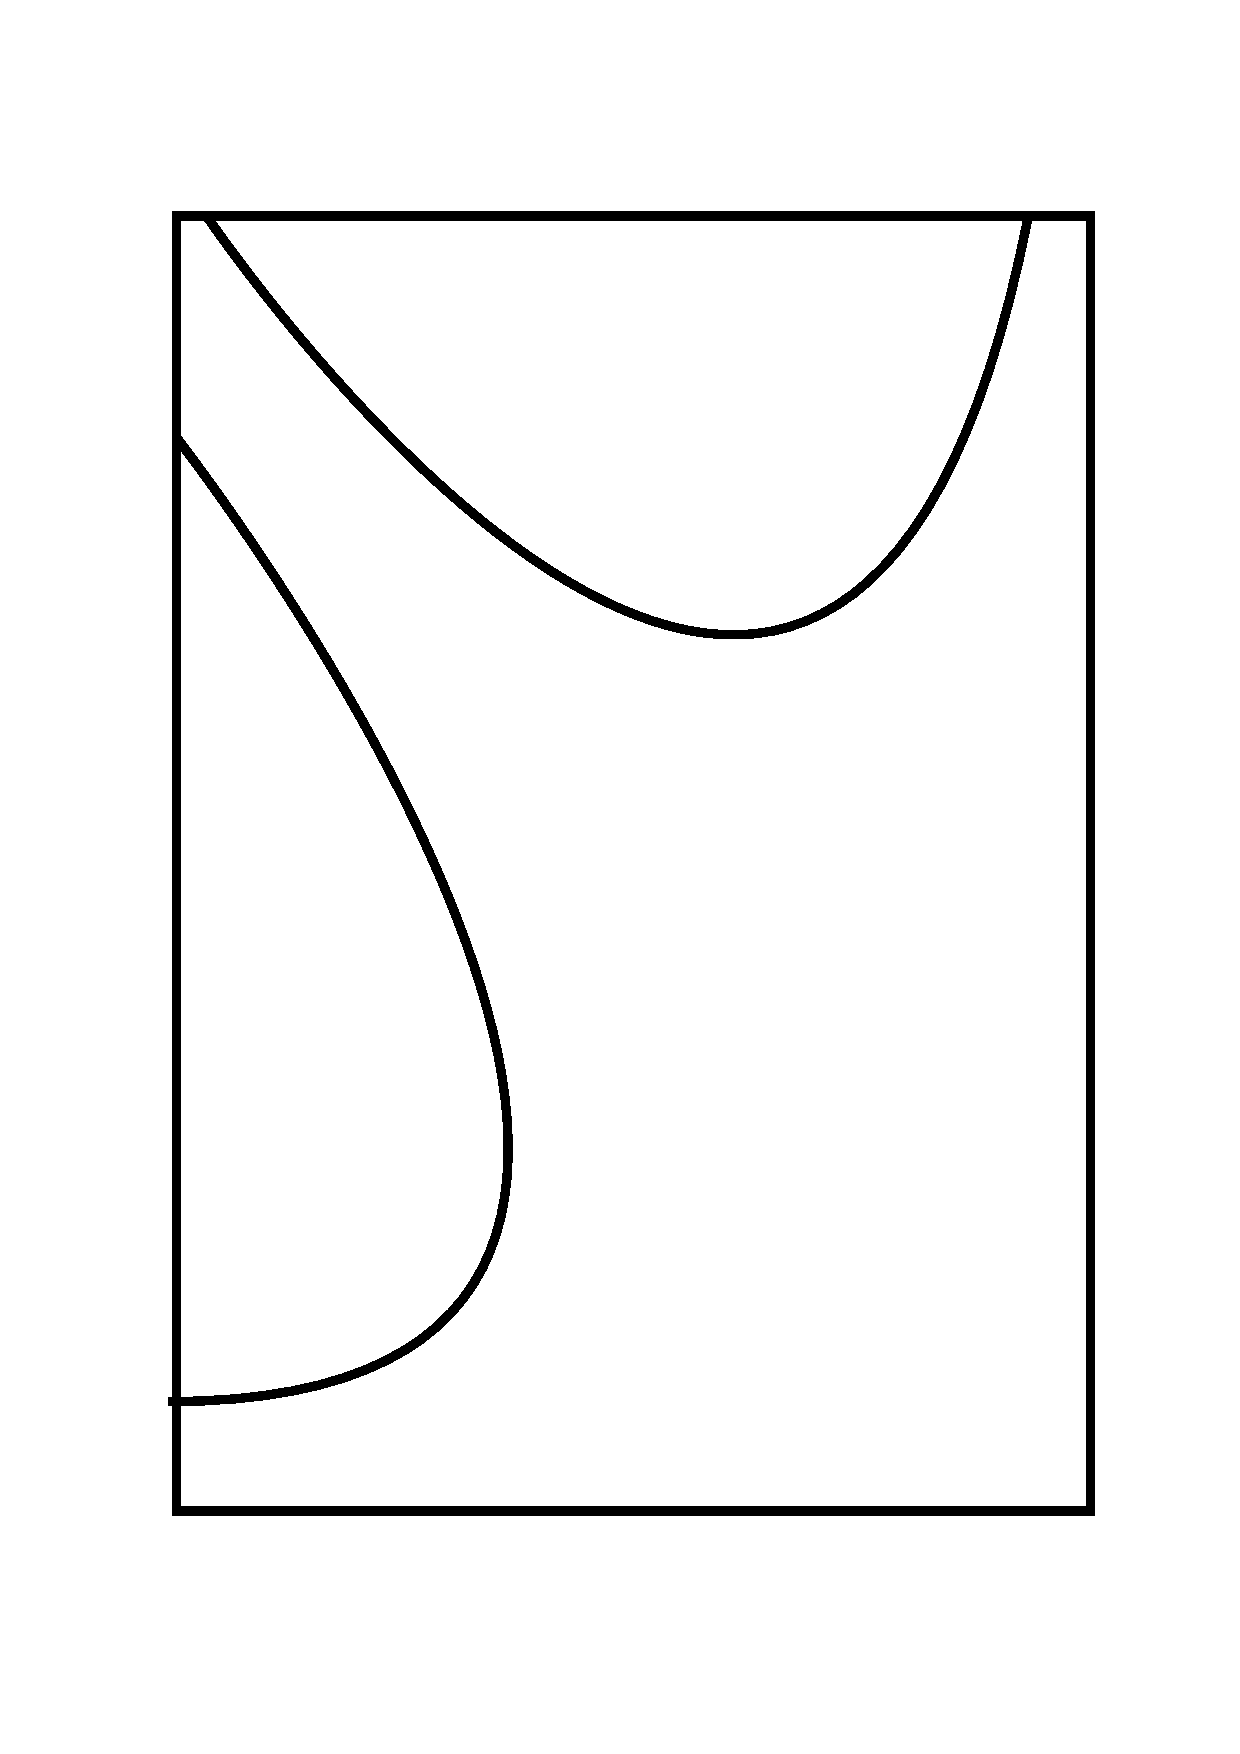
\includegraphics[width = 5cm]{2D1.pdf}
  \caption{2 Dimensions}
  \end{figure}
\end{columns}

\end{frame}



\begin{frame}
{\bf Overview of Results}
\begin{itemize}
  \item Fixed boundary problem is solved efficiently. 
  \item Moving boundary method is generalized to 2 dimensions.
  \item Optimal value and strategy are obtained.
%  \begin{itemize}
%  \item Initial guess.
%  \item Direction and distance of movement.
%  \item The Convergence.
%\end{itemize}
\end{itemize}

\end{frame}




\section{Model}
\begin{frame}
{\bf Model}
\begin{itemize}
  \item One factor model
\begin{equation*}
  dS_t = \kappa ( \mu - \ln S_t)S_t dt + \sigma S_t dW_t
\end{equation*}
\item By Ito's formula, $X_t = \ln(S_t)$ is an Ornstein-Uhlenbeck process,

\begin{equation*}
  dX_t = \kappa ( \alpha - X_t) dt + \sigma dW_t.
\end{equation*}

where $\alpha  = \mu - \sigma^2/(2\kappa)$.
\end{itemize}

\end{frame}

\begin{frame}
{\bf Model}
\begin{itemize}
\item Storage level at time $t$ is $Q_t$. $L_t,U_t$ represent cumulative injections and withdrawals at time $t$.

\begin{equation*}
  dQ_t = dL_t - dU_t
\end{equation*}
\\
\item Admissible if $Q_t \in (Q_{min},Q_{max})~~ \forall t \geq 0$.

\item Costs of injection and withdrawal, $\lambda(X_t,Q_t)$ and $\mu(X_t,Q_t)$, are continuous and bounded.

%In the natural gas example, X_t: leak or use it as the energy for pump. Q_t difficulty.
\end{itemize}

\end{frame}


\begin{frame}
{\bf Model}
% I need to mention that this objective function means that this storage facility is owned by third party instead of producer because there is no benefit of production changing costs.
\begin{itemize}
  \item Objective: to maximize discounted infinite-horizon cash flows.

  \begin{equation}
  \begin{split}
  V(x,q) &= \max_{(L,U) \in \mathcal{U}} \mathbb{E}_{x,q} \left(\int_{0}^{\infty} e^{-\beta t}(e^{X_t} - \mu(Q^1_t))dU_t\right.\\
  &\left.- \int_{0}^{\infty}e^{-\beta t}(e^{X_t} + \lambda(Q^2_t))dL_t\right)
  \end{split}
\end{equation}
% I need to mention this.
where $X_0 =x$ and $Q_0 = q$. %What's more,
%\begin{equation}
%\begin{split}
%  \mu(Q^1_t) = \frac{1}{U_t - U_{t-}}\int_{U_{t-}}^{U_t} \mu(q) dq
%  \end{split}
%\end{equation}
%
%\begin{equation}
%  \lambda(Q^2_t) = \frac{1}{L_t - L_{t-}}\int_{L_{t-}}^{L_t} \lambda(q) dq.
%\end{equation}  
  
\end{itemize}
\end{frame}

\begin{frame}
{\bf The Hamilton-Jacobi-Bellman Equation}
\begin{itemize}
  \item Dynamic programming arguments and Ito's formula yield the Hamilton-Jacobi-Bellman (HJB) equation.
  \begin{equation*}
  \max\left( \mathcal{L} V, \frac{\partial V}{\partial q} - (e^x + \lambda(q)), -\frac{\partial V}{\partial q} + (e^x - \mu(q))\right) = 0
\end{equation*}
with $\mathcal{L}V = \frac{1}{2} \sigma^2 \frac{\partial^2 V}{\partial x^2} + \alpha (\kappa - x) \frac{\partial V}{\partial x} - \beta V$.


  \item A verification theorem assures us that a function that solves the HJB equation is the value function for the original control problem and a policy that achieves this value function is the optimal policy.

\end{itemize}

\end{frame}

\begin{frame}
{\bf The Hamilton-Jacobi-Bellman Equation}
%The first part is the discounted value earned in the future while the second part is the cost I need to pay right now.

\begin{itemize}
\item Assume $V$ is known and the change of policy at one point $(x_0,q_0)$ won't affect it.\\
Now at $(x_0,q_0)$, $\epsilon$ is bought at price $e^{x_0}$. The average buying profit is 
\begin{equation*}
  \frac{\left[V(x_0,q_0 + \epsilon) - V(x_0,q_0)\right] - \epsilon(e^x + \lambda(q))}{\epsilon}
  \stackrel{\epsilon \rightarrow 0}{\longrightarrow} 
  \frac{\partial V}{\partial q} - (e^x + \lambda(q))
\end{equation*}

\item $\mathcal{L}V(x,q)$: holding profit at $(x,q)$.
\item $\frac{\partial V}{\partial q}(x,q) - (e^x + \lambda(q))$: selling profit at $(x,q)$.
\item $-\frac{\partial V}{\partial q}(x,q) + (e^x - \mu(q))$: buying profit at $(x,q)$.

\item HJB equation.
\begin{equation*}
  \max\left( \mathcal{L} V, \frac{\partial V}{\partial q} - (e^x + \lambda(q)), -\frac{\partial V}{\partial q} + (e^x - \mu(q))\right) = 0
\end{equation*}



\end{itemize}

\end{frame}


\begin{frame}
{\bf Holding, Selling and Buying Regions}

\begin{itemize}
  \item The state space $(x,q) \in \mathbb{R}^2_+$ is divided into three kinds of regions.
  \item Holding region: holding profit = 0, selling \& buying profit $<0$
  \item Selling region: selling profit = 0, holding \& buying profit $<0$ 
  \item Buying region: buying profit = 0, holding \& selling profit $<0$
\end{itemize}

\end{frame}

\begin{frame}
{\bf Solving the Fixed Boundary Problem}
\begin{itemize}
  \item In the holding region
  \begin{equation*}
  \frac{1}{2} \sigma^2 \frac{\partial^2 V}{\partial x^2} + \alpha (\kappa - x) \frac{\partial V}{\partial x} - \beta V = 0
\end{equation*}

\item Defining $y = \kappa (x-\alpha)^2/\sigma^2$, we have
\begin{equation*}
  y \frac{\partial^2 V}{\partial y^2} + (0.5 - y) \frac{\partial V}{\partial y} -\frac{\beta}{2\kappa} V = 0
\end{equation*}

which is the Kummer Equation. The solution is the sum of hypergeometric1F1 and the hypergeometricU functions.

\begin{equation*}
\begin{split}
  V(x,q) &= A(q)\text{HyperGeoU}\left(\frac{\beta}{2\kappa},\frac{1}{2},\frac{\kappa}{\sigma^2}(x-\alpha)^2\right) \\
  &+ B(q)\text{HyperGeo1F1}\left(\frac{\beta}{2\kappa},\frac{1}{2},\frac{\kappa}{\sigma^2}(x-\alpha)^2\right)
  \end{split}
\end{equation*}

Boundary conditions can determine $A(q)$ and $B(q)$.

\end{itemize}

\end{frame}

\begin{frame}
{\bf The Structure of Optimal Boundary}

\begin{theorem}
When the price is high enough, regardless of storage, selling is the optimal strategy.
\end{theorem}

% The initial guess for selling boundary is easy. At a high price, set the policies at that level are selling.
% Give an counter example of second intuition.

\end{frame}



\begin{frame}
{\bf The Structure of Optimal Boundary}

\begin{columns}
  \column{0.5\textwidth}
  \begin{figure}[hbt]
  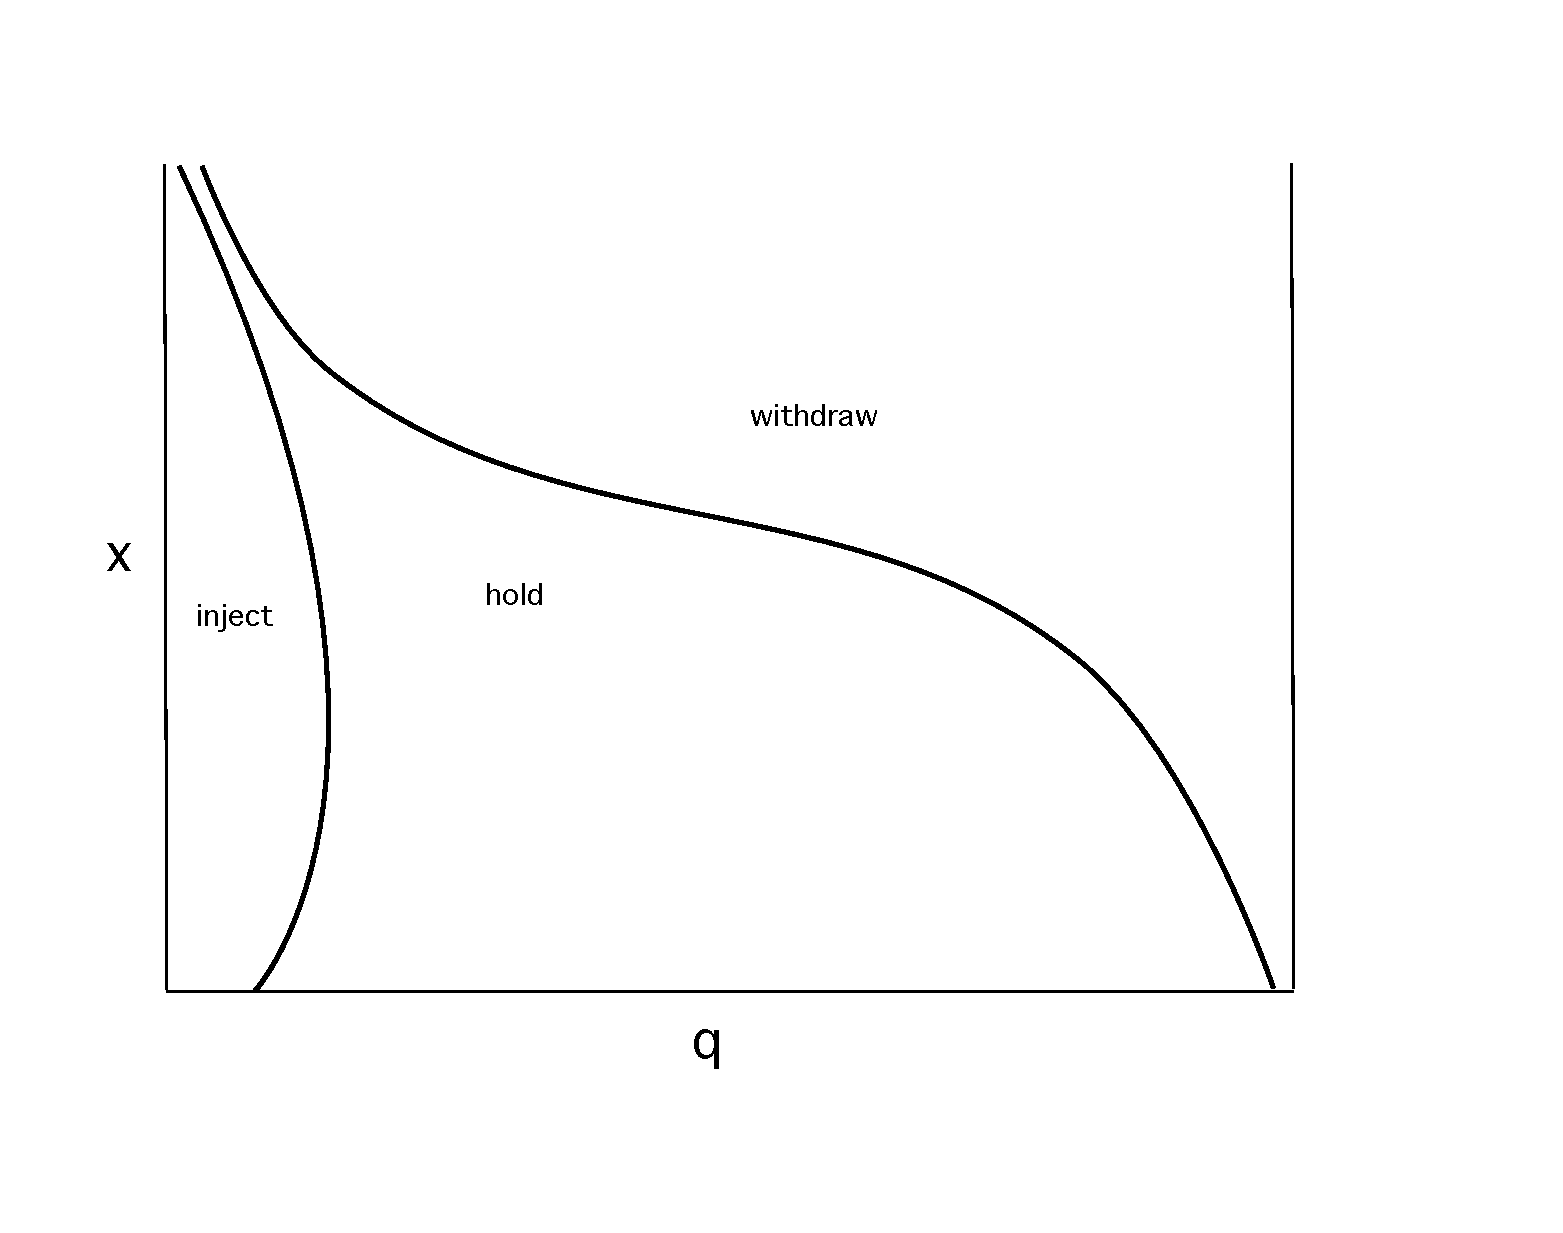
\includegraphics[scale = 0.25]{wonthappen.eps}
  \caption{This won't happen}
  \end{figure}
  \column{0.5\textwidth} 
   \begin{theorem}
    Under optimal policy, there won't exist $x$ and $q_1 \neq q_2$ such that buying happens at $(x,q_1)$ while selling happens at $(x,q_2)$.
    \end{theorem}
\end{columns}
%Move the fixed boundary problem here. As long as fixed problem is easy to solve, we can use moving boundary method.


%\only<1>{Long: Transaction cost will only change selling(buying) to holding. It won't change selling to buying or reverse.}
\end{frame}

\section{Moving Boundary Method}
\begin{frame}
{\bf The Moving Boundary Method}

\begin{columns}
   \column{0.4\textwidth} 
\begin{itemize}
  \item Challenges
  \begin{itemize}
  \item Initial guess.
  \item 2 dimensions.
\begin{itemize}
  \item Direction.
  \item Distance.
\end{itemize}
  \end{itemize}
\end{itemize}
  \column{0.7\textwidth}
\only<2>{\begin{figure}[hbt]
  \includegraphics[scale = 0.4]{0step.eps}
  \caption{Initial Guess}
  \end{figure}}
\only<3>{\begin{figure}[hbt]
  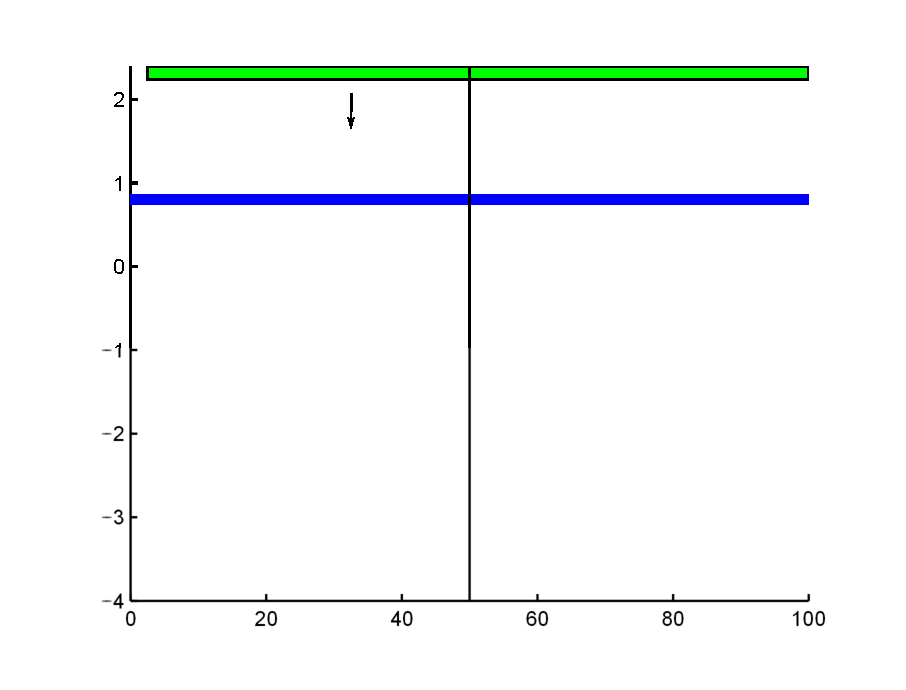
\includegraphics[scale = 0.4]{Where2Move0step.eps}
  \caption{Initial Guess}
\end{figure}}
  \end{columns}
\end{frame}

\begin{frame}
{\bf Algorithm}
\begin{enumerate}
  \item Begin with selling at very high price for all $q>0$.
  \item Move selling and buying boundaries along price $x$ alternatively until convergence. 
%  \begin{itemize}
%  \item  The initial guess of buying is generated in this procedure.
%  \item  Each time move to the point that generates highest positive profit.
%\end{itemize}



\end{enumerate}

\end{frame}


%\begin{frame}
%{\bf How does Moving Boundary Method Work?}
%
%%todo: use movie instead of pictures to show this. At first show it extremely slow then increase the speed toward the end.
%\centering
%\only<1>{
%\begin{figure}[hbt]
%  \includegraphics[scale = 0.5]{0step.eps}
%  \caption{Initial Policy}
%\end{figure}
%}
%
%%%\only<2>{
%%%\begin{figure}[hbt]
%%%  \includegraphics[scale = 0.5]{1step.eps}
%%%  \caption{1st Step}
%%%\end{figure}
%%%}
%%%\only<3>{
%%%\begin{figure}[hbt]
%%%  \includegraphics[scale = 0.5]{2step.eps}
%%%  \caption{2nd Step}
%%%\end{figure}
%%%}
%%%\only<4>{
%%%\begin{figure}[hbt]
%%%  \includegraphics[scale = 0.5]{3step.eps}
%%%  \caption{3rd Step}
%%%\end{figure}
%%%}
%
%\only<2>{
%\begin{figure}[hbt]
%  \includegraphics[scale = 0.5]{9step.eps}
%  \caption{9th Step}
%\end{figure}
%}
%
%\only<3>{
%\begin{figure}[hbt]
%  \includegraphics[scale = 0.5]{10step.eps}
%  \caption{10th Step}
%\end{figure}
%}
%
%\only<4>{
%\begin{figure}[hbt]
%  \includegraphics[scale = 0.5]{11step.eps}
%  \caption{11th Step}
%\end{figure}
%}
%
%\only<5>{
%\begin{figure}[hbt]
%  \includegraphics[scale = 0.5]{12step.eps}
%  \caption{12th Step}
%\end{figure}
%}
%
%\only<6>{
%\begin{figure}[hbt]
%  \includegraphics[scale = 0.5]{13step.eps}
%  \caption{13th Step}
%\end{figure}
%}
%
%\only<7>{
%\begin{figure}[hbt]
%  \includegraphics[scale = 0.5]{14step.eps}
%  \caption{14th Step}
%\end{figure}
%}
%
%\only<8>{
%\begin{figure}[hbt]
%  \includegraphics[scale = 0.5]{laststep.eps}
%  \caption{Last Step}
%\end{figure}
%}
%
%\end{frame}

\begin{frame}
{\bf Distance}
% Check the result with Kumar. Is the maximum point is moved to.
Because there is \textit{No Coming Back}, overshooting must be avoided. \\

{\large Sell}
%todo: put a black dot in the graph and an arrow there.
\begin{columns}
\column{0.5\textwidth}
%\only<1>{
\begin{figure}[hbt]
  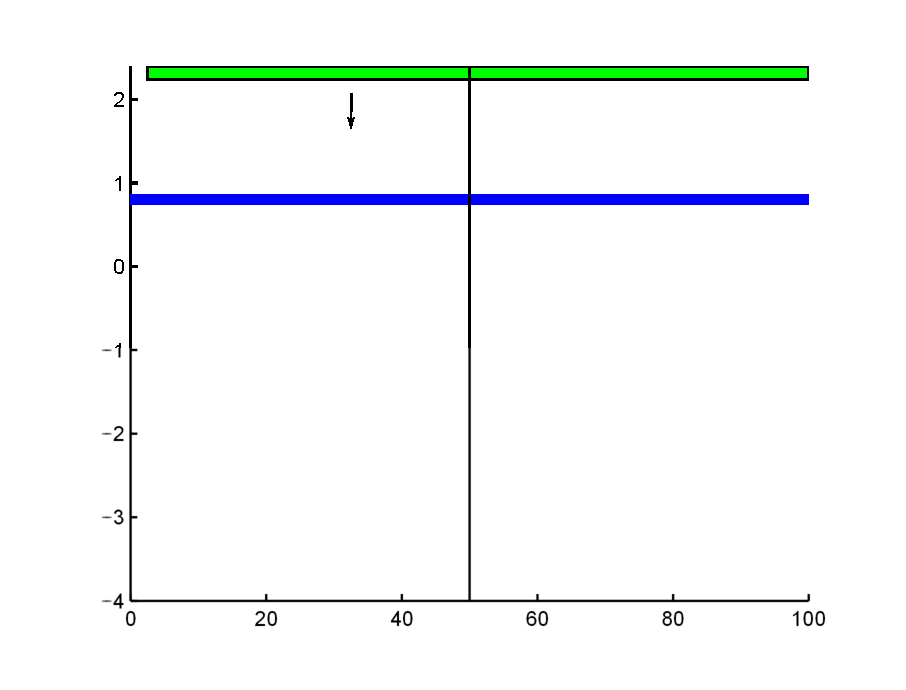
\includegraphics[scale = 0.4]{Where2Move0step.eps}
  \caption{Current Policy}
\end{figure}
%}
  \column{0.5\textwidth} 
  \only<2>{
\begin{figure}[hbt]
  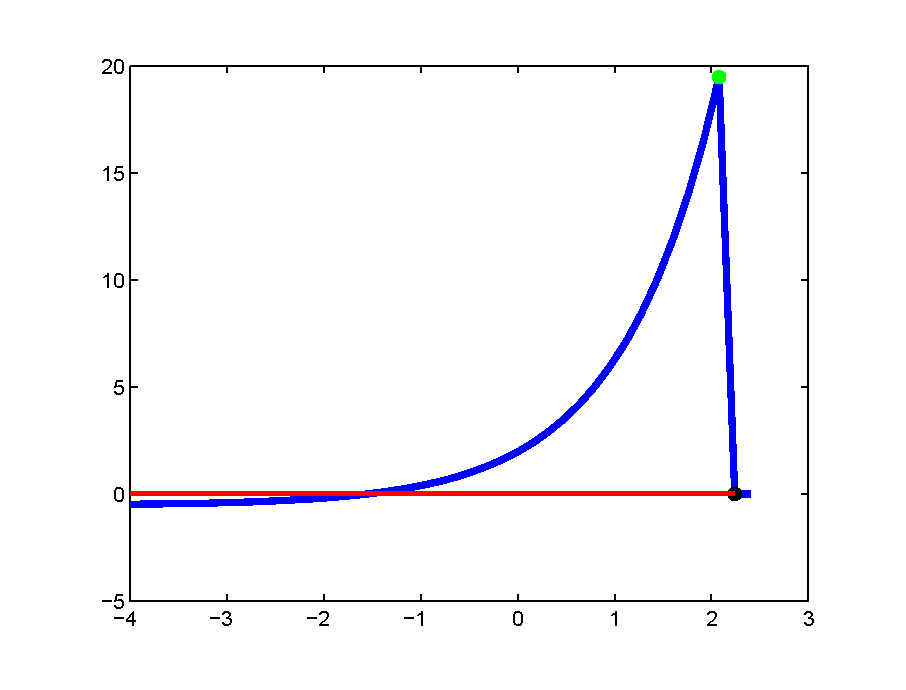
\includegraphics[scale = 0.4]{Where2MoveSell.eps}
  \caption{Selling Profit}
\end{figure}
}
\only<3>{
\begin{figure}[hbt]
  \includegraphics[scale = 0.4]{Where2Move1step.eps}
  \caption{After Movement}
\end{figure}
}
\end{columns}
\end{frame}

\begin{frame}

{\large Buy}
%todo: put a black dot in the graph and an arrow there.
\begin{columns}
\column{0.5\textwidth}
%\only<1>{
\begin{figure}[hbt]
  \includegraphics[scale = 0.4]{Where2Move13step.eps}
  \caption{Current Policy}
\end{figure}
%}
  \column{0.5\textwidth} 
\only<2>{
\begin{figure}[hbt]
  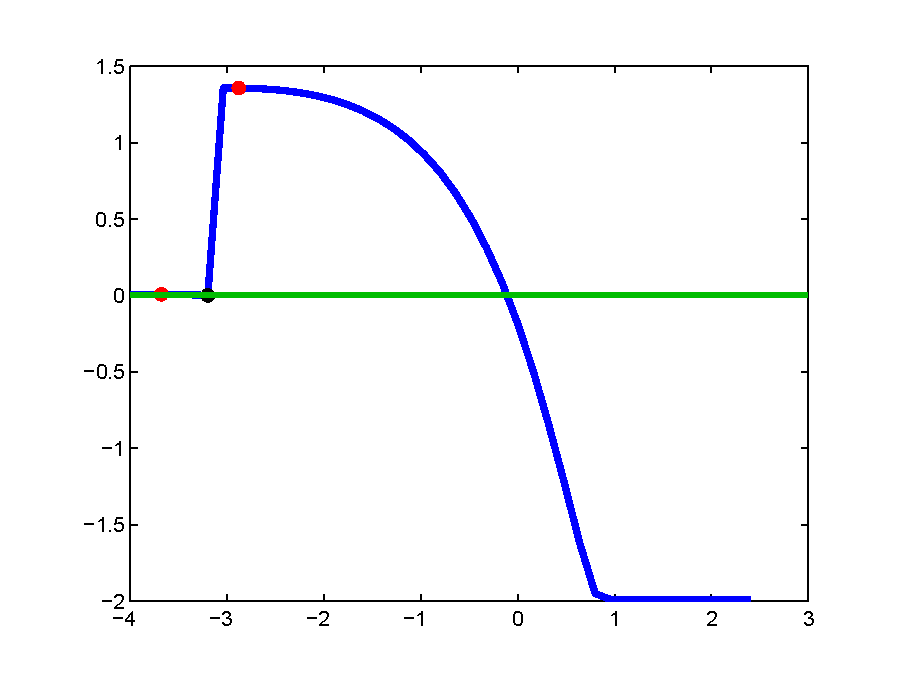
\includegraphics[scale = 0.4]{Where2MoveBuy.eps}
  \caption{Buying Profit}
\end{figure}
}
\only<3>{
\begin{figure}[hbt]
  \includegraphics[scale = 0.4]{Where2Move14step.eps}
  \caption{After Movement}
\end{figure}
}
\end{columns}
\end{frame}


\begin{frame}
{\bf Proof of Convergence}
\begin{Theorem}
Each movement improves value function.
\end{Theorem}
\begin{columns}
   \column{0.5\textwidth} 
  \begin{figure}[hbt]
  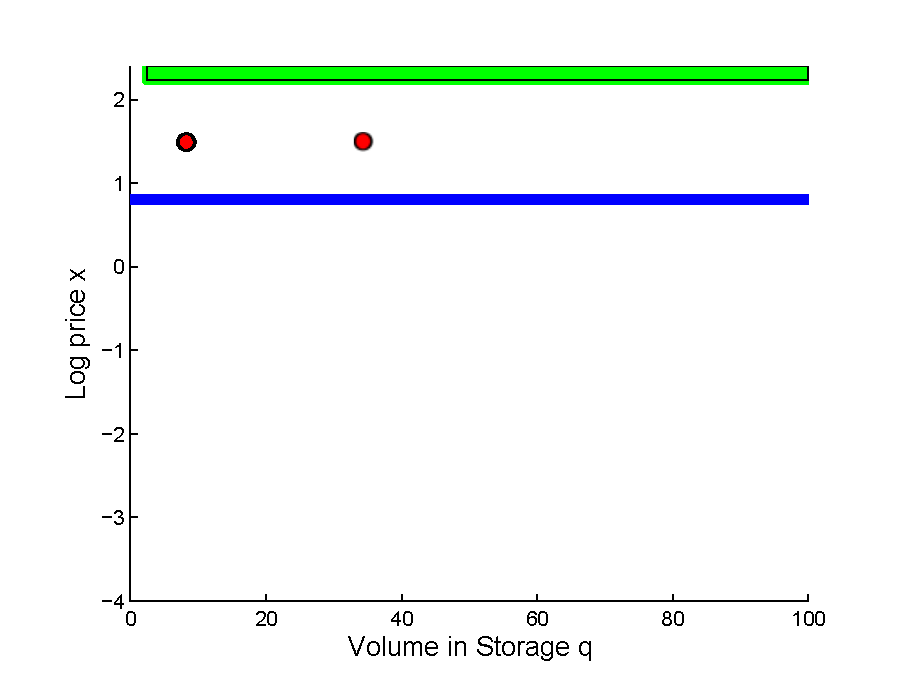
\includegraphics[scale = 0.4]{0Converge.eps}
  \caption{Initial Guess}
  \end{figure}
  \column{0.5\textwidth}
  \begin{figure}[hbt]
  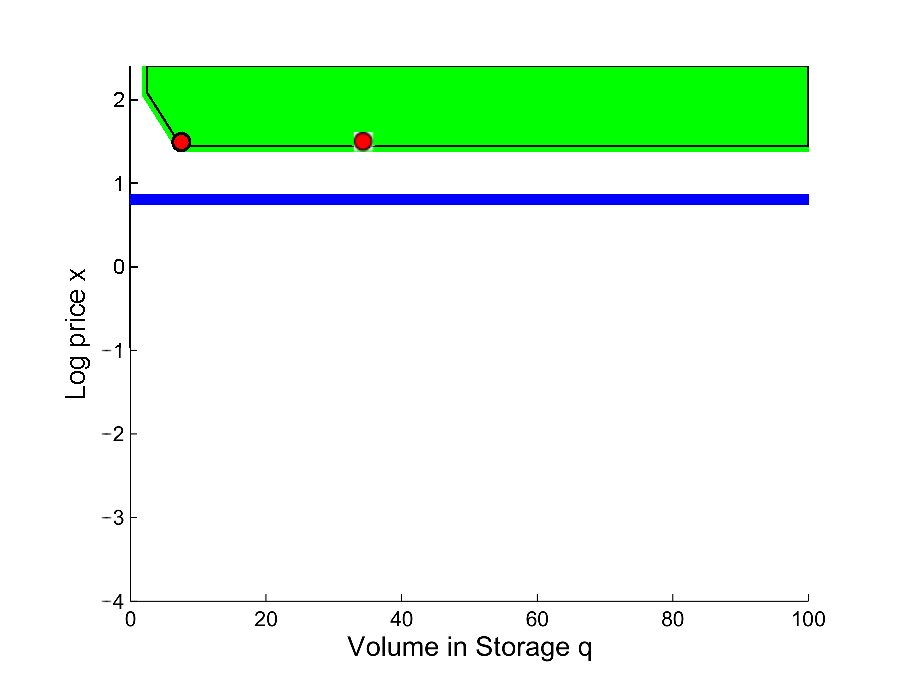
\includegraphics[scale = 0.4]{9Converge.eps}
  \caption{Initial Guess}
\end{figure}
\end{columns}

\end{frame}

%Todo: give more intuition about this theorem. Make sure with Kumar that this is the right way.

\begin{frame}
{\bf Proof of Convergence}
% What does \Delta V_q > 0 mean?
\begin{Theorem}
The boundaries can be kept moving.
\end{Theorem}
\end{frame}


\begin{frame}
{\bf Extensions}

\begin{itemize}
  \item Seasonality and Finite time.
  \item Depreciation.
  \item Random injection and withdrawal.
\end{itemize}

\end{frame}




\end{document} 